% Section "kepler" (paper section 10). Owner group: kepler.
% Sources: research/tracks/philosophy/notes-final.md section 4 (Props 4.1-4.4, sections 4.3-4.5) with its
% status table (section 11) and refuted/withdrawn list (11.1; nothing refuted is printed); laws section 3.6 and
% Prop 5.5; synthesis H11, 2.6, 5.5 (statement discipline). Proofs, law texts, full tables, witnessing elements,
% and the residual and distance tables (moved there for the page budget): sections/app-kepler.tex.
% Figure 1 is drawn below in TikZ from the saved outputs of the Mars-pool computation (no recomputation):
% switch points = the minimax errors of tab:kepler:minimax; MAP rows = table A4 of the saved output; dots = the
% 13 precisions at which the posterior was computed; x = 4 log10(720'/delta).
% Local symbol renames (logged): the record's theta_K3, theta_pos -> \zeta_{K3}, \zeta_{pos} (theta is the
% longitude); d(b,t,v,delta) -> Near(b,t,v,delta); Delta_K3 -> s_K3 (as the saving s of prop:laws:K3).
\section{A worked example: Kepler and Newton}\label{sec:kepler}

We work through one example: Kepler's laws of planetary motion, the theories of the motion of Mars that preceded the ellipse, and what Newton's theory adds. It shows that what a law says depends on the data language (\cref{sec:kepler:content}); that in a proof-requiring posterior over the historical theories of Mars the data decide which theories are compatible, while among compatible theories, on noise-free data, the language of the law texts decides (\cref{sec:kepler:pool}); and that the gain of a successor theory need not lie in a better fit to the old data (\cref{sec:kepler:newton}). The data of every computation are the plan94 ephemeris of the ERFA library, so \emph{every arcminute figure in this section is an error against plan94, not against the sky}. The code is in the accompanying repository; \cref{app:kepler} gives the proofs, the law texts, the full tables and the elements that witness each fit.

% ------------------------------------------------------------------
\subsection{The language and the data}\label{sec:kepler:language}

\begin{definition}[the Kepler languages and theories]\label{def:kepler:language}
\status{definition}\src{philosophy \S4.1}
\leavevmode
\begin{enumerate}[label=(\roman*),leftmargin=*,itemsep=1pt]
\item \emph{Data languages.} Sorts bodies and reals; body constants Sun, Me, Ve, Ea, Ma, Ju, Sa, Mo; a predicate Planet. The \emph{heliocentric language} $\mathcal L_{\rm hel}$ has the heliocentric ecliptic longitude, latitude and distance $\theta(b,t),\beta(b,t),r(b,t)$ of body $b$ at time $t$ (for the Moon, geocentric); its direction-only part $\mathcal L_{\rm dir}$ omits $r$. The \emph{geocentric language} $\mathcal L_{\rm geo}$ has $\theta_g(b,t),\beta_g(b,t)$, giving the direction $\mathrm{dir}_g(b,t)\in S^2$: a modern idealisation of Tycho's data (our data are geometric plan94 positions, without aberration or light time).
\item \emph{Background.} $B$: the axioms of real closed fields with $\sin$, $\cos$, $\pi$, and enough true analysis to prove the numerical bounds used (rational-function bounds of the kind MetiTarski proves \citep{akbarpour2010metitarski}). The theory of the reals with $\sin$ is undecidable ($\sin(\pi x)=0$ defines $\mathbb Z$), so $B$ is a sound decidable fragment; each result names the true sentences it needs.
\item \emph{Kepler's first two laws} $\mathrm{K12}$, in the theoretical vocabulary of heliocentric positions $\mathbf r(b,t)\in\mathbb R^3$ and the elements $a,e,i,\Omega,\varpi,M_0,P$ (functions from bodies to reals: semi-major axis, eccentricity, inclination, node, longitude of perihelion, mean anomaly at the epoch, period): for every planet $b$ and every $t$, with $M:=M_0(b)+2\pi t/P(b)$, there is $\psi$ with $\psi-e(b)\sin\psi=M$ and $\mathbf r(b,t)=\mathrm{Rot}(b)\big(a(b)(\cos\psi-e(b)),\,a(b)\sqrt{1-e(b)^2}\sin\psi,\,0\big)$, where $\mathrm{Rot}(b)$ is the rotation given by $i(b),\Omega(b),\varpi(b)$; moreover $0\le e(b)<1$, $a(b),P(b)>0$ and $\mathbf r(\mathrm{Sun},t)=0$. Over $\mathcal L_{\rm geo}$, $\mathrm{K12}$ also contains the frame convention $i(\mathrm{Ea})=0$ and the \emph{bridge}: $\mathrm{dir}_g(b,t)$ is the unit vector of $\mathbf r(b,t)-\mathbf r(\mathrm{Ea},t)$ if this is nonzero, and the north ecliptic pole $\mathbf z$ otherwise.
\item \emph{Kepler's third law} $\mathrm{K3}$: $P(b)^2a(b')^3=P(b')^2a(b)^3$ for all planets $b,b'$.
\item \emph{Elements} (initial conditions): numerals, or intervals, for the elements of a body. \emph{Data}: true interval sentences $\mathrm{Near}(b,t,\mathbf v,\delta)$, ``the direction of $b$ at $t$ lies within angle $\delta$ of $\mathbf v$'' ($\mathrm{Near}_g$ for geocentric directions), with numerals for $t,\mathbf v,\delta$, and, where available, $r(b,t)\in[r_1,r_2]$. \emph{Questions} (\cref{def:setting:questions}): covers by such sentences (``where is Mars at $t$, to within $2'$?''), and structural questions, which the laws answer without elements (is the orbit planar; does the direction return periodically; are equal areas swept in equal times).
\end{enumerate}
\end{definition}

Laws alone answer no position question;\footnote{Even the Ramsey sentence of $\mathrm{K12}\cup\mathrm{K3}$, together with any background true in $\mathbb R$, entails (in second-order semantic consequence) no datum $\mathrm{Near}(b,t,\mathbf v,\delta)$ with $\delta<\pi$ (\cref{prop:kepler:ramsey}).} laws with elements do. If the elements are put into the antecedents of conditional questions (\cref{def:setting:questions}), the laws alone answer every such question, and in the solar-system model of \cref{prop:laws:questions} no steeper MAP then contains elements. This is where the distinction between laws and initial conditions sits formally.

% ------------------------------------------------------------------
\subsection{What the laws say, and in which language}\label{sec:kepler:content}

\begin{proposition}[no content in heliocentric directions]\label{prop:kepler:helio}
\status{proved}\src{philosophy Prop 4.2}
For every $B$ that contains the axioms of real closed fields, $\mathrm{K12}$ and $\mathrm{K12}\cup\mathrm{K3}$ have the same $\mathcal L_{\rm dir}$-consequences.
\end{proposition}

\emph{Proof idea.} A Kepler direction does not depend on $a$. Replacing each $a(b)$ in a model of $B\cup\mathrm{K12}$ by $(k^2P(b)^2/4\pi^2)^{1/3}$ keeps every direction and makes $\mathrm{K3}$ true (\cref{sec:kepler:proofs}).

\begin{proposition}[content in geocentric directions]\label{prop:kepler:geo}
\status{proved; computed}\src{philosophy Prop 4.3}
Let $\chi_{\rm opp}$ be the $\mathcal L_{\rm geo}$-sentence $\exists t\ \mathrm{dir}_g(\mathrm{Ma},t)\ne-\mathrm{dir}_g(\mathrm{Sun},t)$ (``Mars is not permanently in opposition'').
\begin{enumerate}[label=(\alph*),leftmargin=*,itemsep=0pt]
\item $\chi_{\rm opp}$ holds in every model of $\mathrm{K12}\cup\mathrm{K3}$ whose real sort is $\mathbb R$. Hence $B\cup\mathrm{K12}\cup\mathrm{K3}\vdash\chi_{\rm opp}$ for every $B$ that contains the two true sentences $\zeta_{\rm K3}$ and $\zeta_{\rm pos}$ of the real field with $\sin$ and $\cos$ given in \cref{sec:kepler:proofs}.
\item For every $B$ true in $\mathbb R$, $B\cup\mathrm{K12}\nvdash\chi_{\rm opp}$.
\end{enumerate}
\end{proposition}

\emph{Proof idea.} (b) Circular coplanar orbits with equal periods and phases, Mars at distance $\rho>1$, satisfy $\mathrm{K12}$ (which relates no bodies), violate $\mathrm{K3}$ and keep Mars in opposition. (a) Over $\mathbb R$, a Mars permanently in opposition stays on the ray from the Sun through the Earth, and Kepler's second law forces $\mathbf r(\mathrm{Ma},t)=\kappa\,\mathbf r(\mathrm{Ea},t)$ with a constant $\kappa>1$: equal periods, different semi-major axes, against $\mathrm{K3}$. $\zeta_{\rm K3}$ states this about the elements, and $\zeta_{\rm pos}$ (the Earth is never at the Sun) lets the argument cover non-standard models.

The sentence $\chi_{\rm opp}$ is odd (its negation describes a fantastic world); it only shows that the geocentric language can register $\mathrm{K3}$. The natural form of $\mathrm{K3}$'s content is this:

\begin{proposition}[what K3 does in geocentric directions]\label{prop:kepler:K3worth}
\status{proved; computed}\src{philosophy Prop 4.4}
Let $\mathrm{Num}^-$ be numerals for all elements of the Earth and Mars except $a(\mathrm{Ma})$, with $a(\mathrm{Ea})=1$. Let $\mathbf F(t)$ be Mars's heliocentric position computed from $\mathrm{Num}^-$ with semi-major axis $1$, so that $\mathbf r(\mathrm{Ma},t)=\rho\,\mathbf F(t)$ with $\rho:=a(\mathrm{Ma})$, and let $\mathbf u(t)$ be the unit vector of $\mathbf r(\mathrm{Ea},t)$.
\begin{enumerate}[label=(\alph*),leftmargin=*,itemsep=0pt]
\item $\mathrm{K12}\cup\mathrm{K3}\cup\mathrm{Num}^-$ fixes $\rho=(P(\mathrm{Ma})/P(\mathrm{Ea}))^{2/3}$ and hence every geocentric direction of Mars: it proves $\mathrm{Near}_g(\mathrm{Ma},t,\mathbf v,\delta)$ whenever the computed direction lies within $\delta$ of $\mathbf v$ and $B$ proves the numerical bound involved.
\item $\mathrm{K12}\cup\mathrm{Num}^-$ leaves $\rho$ free. At every $t$ at which $\mathbf r(\mathrm{Ea},t)$ and $\mathbf F(t)$ are not parallel, the geocentric directions of Mars at $t$ in the models of $\mathrm{K12}\cup\mathrm{Num}^-$ over $\mathbb R$ (with $\rho$ ranging over $(0,\infty)$) form the open great-circle arc from $-\mathbf u(t)$, the direction of the Sun, to $\mathbf F(t)/\lvert\mathbf F(t)\rvert$; its length $\alpha(t)\in(0,\pi)$ is the angle between these two directions. So for every $B$ true in $\mathbb R$, $B\cup\mathrm{K12}\cup\mathrm{Num}^-$ proves no datum $\mathrm{Near}_g(\mathrm{Ma},t,\mathbf v,\delta)$ with $\delta<\alpha(t)/2$.
\end{enumerate}
\end{proposition}

\emph{Proof idea.} As $\rho$ runs over $(0,\infty)$, the vector $\rho\mathbf F(t)-\mathbf r(\mathrm{Ea},t)$ runs along an open ray that misses the origin, so its direction sweeps the open arc; an arc of length $\alpha$ lies in no cap of radius less than $\alpha/2$ (\cref{sec:kepler:proofs}).

\begin{example}[K3's worth against its cost; a computation]\label{ex:kepler:K3cost}
\status{computed (conditional on the code; the extrapolation and the compact-code threshold are estimates)}\src{philosophy \S4.4 Part B; laws Prop 5.5(b)}
Given the other elements, $\mathrm{K3}$'s geocentric content is thus exactly $\rho$, and it is large: over 1580--1600 the median of $\alpha(t)$ is $90^\circ$ (5th and 95th percentiles $9.5^\circ$ and $170^\circ$). Take as data the daily geocentric longitudes of Mars over 1580.0--1600.0 at a common tolerance $\delta$, and Kepler ellipses for the Earth and Mars with $\rho\in[0,4)$ free or given by $\mathrm{K3}$. With fixed-length numerals for the elements, the posterior odds for $\mathrm{K3}$ are $2^{s_{\rm K3}(\delta)-\lvert\mathrm{K3}\rvert}$, where $\lvert\mathrm{K3}\rvert$ is the length of its text and $s_{\rm K3}(\delta):=\log(4\,\mathrm{Vol}_8(\delta)/\mathrm{Vol}_9(\delta))$ ($\mathrm{Vol}_8,\mathrm{Vol}_9$ the volumes of the compatible element regions with and without $\mathrm{K3}$) is what $\mathrm{K3}$ saves (\cref{sec:kepler:K3details}). A computation gives $s_{\rm K3}=11.3$, $12.3$, $13.4$, $14.7$ bits at $\delta=8'$, $4'$, $2'$, $1'$, about one more bit per halving of $\delta$, as for any real-valued element; $\mathrm{K3}$ costs $0.005'$ of fit. Its text costs $375$ bits in the syntax S1 of \cref{sec:kepler:pool} (brackets counted), $165$ in Polish notation and $115$ in a compact Polish code; it is paid once and saves $s_{\rm K3}(\delta)$ bits per body whose size it fixes. By \cref{prop:laws:K3} (with the law in place, at exchange rate $1$; a comparison of law choices, not membership of a steeper MAP), $\mathrm{K3}$ pays once it fixes the sizes of about $25$--$33$, $11$--$15$ or $8$--$10$ bodies in the three codes, while the five planets other than the Earth give about $55$--$75$ bits if each saves about as much as Mars (an extrapolation; we computed Mars only). So in none of these codes does compression alone select $\mathrm{K3}$ at Kepler's precision. This is conditional on the code: under the universal prior the relevant cost is the complexity of $\mathrm{K3}$ given the rest of the theory, which these computations do not determine.
\end{example}

$\mathrm{K3}$ is thus a law about initial conditions, worth what it saves on the elements of the bodies it relates. This depends on Kepler's kinematic parametrisation, with the period and the semi-major axis both free; in a state-space parametrisation $\mathrm{K3}$ fixes the mean motion from the energy, a different question, and in Newton's theory the third law, with its mass correction, follows from the one law that does all the other work and costs nothing extra.

% ------------------------------------------------------------------
\subsection{How wrong Kepler's laws are}\label{sec:kepler:wrong}

Kepler's laws are approximately true, with an error that grows with the domain: one fixed ellipse, fitted by least squares, misses Mars by $1.6'$--$1.9'$ over 12--30 years, $3.61'$ over a century and $51.8'$ over 2000 years, and the Moon by $1.1^\circ$ within a month (\cref{tab:kepler:residuals} in \cref{sec:kepler:data}). The third-law ``constant'' $q:=(2\pi/P)^2a^3/k^2$ ($k$ Gauss's constant) differs between planets at the $10^{-3}$ level: Jupiter's fitted value matches the Newtonian two-body value $1+m/M$, while Saturn's needs Jupiter's pull. Yet at the precision of Tycho's data $\mathrm{K3}$'s own error is invisible: an exact $\mathrm{K3}$ calibrated on the Earth misplaces Jupiter and Saturn geocentrically by at most $0.23'$ and $0.19'$ over 1580--1600. \emph{The error budget:} by the accuracy that the documentation of ERFA's routine quotes, plan94's own error in the heliocentric longitude of Mars over 1580--1600 is at most about $0.43'$; for Jupiter and Saturn it is larger, and their 12-year residuals measure the ellipse against plan94 rather than the sky (\cref{sec:kepler:data}).

% ------------------------------------------------------------------
\subsection{The proof-requiring posterior over the historical Mars pool}\label{sec:kepler:pool}

\paragraph{The pool and the data.} We take a hand-picked pool of five forms of theory for the motion of Mars, as heliocentric reconstructions (the earlier historical models were geocentric and also represented the Earth's motion): the circle about the Sun (2 elements), the eccentric circle of Hipparchus (4), Ptolemy's bisected equant (4), Kepler's vicarious hypothesis (5) and the ellipse $\mathrm{K12}$ (4) (\cref{sec:kepler:pooldetails}). The data are the 7306 daily plan94 heliocentric longitudes $v_i$ of Mars over 1580.0--1600.0, in the best plane through the Sun, each stated as the interval sentence ``$\theta(t_i)$ lies within $\delta$ of $v_i$'': the guaranteed-tolerance regime of \cref{prop:laws:tolerance} with zero measurement error, the noise-free special case. A form with suitable elements proves every datum iff $\delta$ is at least its \emph{minimax error}, the least over elements of its largest error (\cref{tab:kepler:minimax}); here this is an upper bound witnessed by elements and reproduced to four decimals by an independent search (only the circle's is proved optimal). The equant's $8'$ is intrinsic (it remains against an exact ellipse), close to the famous discrepancy of about eight minutes of arc in Kepler's \emph{Astronomia Nova} \citep{kepler1992new}; more than half of the vicarious hypothesis's $1.41'$ is perturbation error shared with the ellipse, and the $0.34'$ between the two is of the size of plan94's error, so against the sky their ordering rests on the errors against an exact ellipse.

\paragraph{The posterior.} A theory is a law text in one of three syntaxes plus fixed-length 64-bit numerals for its elements; the proof-requiring rule of $\MA$ (\cref{def:setting:MA}), with the universal machine replaced by this code, gives it weight $2^{-\text{length}}$ if it proves every datum (it is then consistent with the data) and $0$ otherwise. Summing over numerals, form $\mathsf F$ has weight proportional to $2^{-(\lvert\mathrm{LAW}_{\mathsf F}\rvert_S+\Occ_{\mathsf F}(\delta))}$, with $\lvert\mathrm{LAW}_{\mathsf F}\rvert_S$ the length of its law text in syntax $S$ and $\Occ_{\mathsf F}(\delta):=-\log(\mathrm{Vol}_{\mathsf F}(\delta)/\prod\text{ranges})$ its \emph{Occam factor}, $\mathrm{Vol}_{\mathsf F}(\delta)$ being the volume of the elements with which $\mathsf F$ proves all the data (the term is MacKay's \citep{mackay1992bayesian}; \citealp{jefferys1992ockham} read Bayes factors this way for Mercury's perihelion). The syntaxes are \emph{S1}, arithmetic ($+,-,\cdot,/,\sin,\cos,\mathrm{atan2},\sqrt{\ }$, the numerals $0,1,2$, quantifiers); \emph{S2}, epicyclic (S1 with primitives for unit vectors, directions, and the point where a ray meets a circle); and \emph{S3}, Keplerian (S1 with the true anomaly as a function of the eccentricity and the mean anomaly).

\begin{table}[t]
\centering\small\crefabbrev
\begin{minipage}[t]{0.35\textwidth}\centering
\caption{Minimax errors of the Mars pool, 1580--1600 (arcminutes): against plan94 (upper bounds witnessed by elements, \cref{sec:kepler:pooldetails}), and against an exact ellipse.}\label{tab:kepler:minimax}
\status{computed (upper bounds witnessed by elements, reproduced by an independent search; global optimality not proved)}\src{philosophy \S4.3--\S4.4}
\setlength{\tabcolsep}{4pt}
\begin{tabular}{@{}lrrr@{}}
\toprule
form & $k$ & plan94 & exact\\
\midrule
circle & 2 & 640.79 & --\\
eccentric & 4 & 23.05 & 22.34\\
equant & 4 & 8.17 & 7.43\\
vicarious & 5 & 1.41 & 0.62\\
ellipse & 4 & 1.07 & 0\\
\bottomrule
\end{tabular}
\end{minipage}\hfill
\begin{minipage}[t]{0.62\textwidth}\centering
\caption{The proof-requiring posterior over the Mars pool: law-text lengths and Occam factors (bits; ``--'': $\delta$ below the minimax error; all values in \cref{sec:kepler:pooldetails}). A form's weight is $\propto2^{-(\text{text}+\text{Occam factor})}$. $\mathrm{K3}$'s text: 375 bits in S1 and S3, 450 in S2.}\label{tab:kepler:map}
\status{computed}\src{philosophy \S4.4 Part A}
\setlength{\tabcolsep}{4pt}
\begin{tabular}{@{}lrrrrr@{}}
\toprule
& circle & eccentric & equant & vicarious & ellipse\\
\midrule
text, S1 & 155 & 445 & 990 & 990 & 545\\
text, S2 & 186 & 342 & 450 & 468 & 654\\
text, S3 & 155 & 445 & 990 & 990 & 260\\
\midrule
$\Occ_{\mathsf F}(720')$ & 20.93 & 20.24 & 21.20 & 22.77 & 21.18\\
$\Occ_{\mathsf F}(30')$ & -- & 45.38 & 40.35 & 42.83 & 39.65\\
$\Occ_{\mathsf F}(9')$ & -- & -- & 57.34 & 51.78 & 46.81\\
$\Occ_{\mathsf F}(1.6')$ & -- & -- & -- & 74.54 & 59.93\\
\bottomrule
\end{tabular}
\end{minipage}
\end{table}

\begin{figure}[t]
\centering
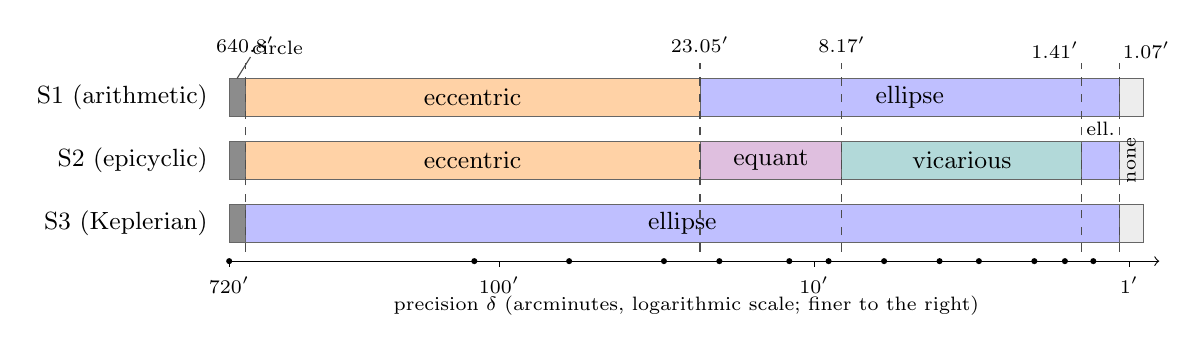
\begin{tikzpicture}[x=1cm,y=0.8cm,font=\small]
% x = 4 log10(720/delta); switch points at the minimax errors 640.79, 23.05, 8.17, 1.41, 1.07 (arcmin)
\def\keplerxc{0.202}\def\keplerxe{5.979}\def\keplerxq{7.781}\def\keplerxv{10.829}\def\keplerxl{11.306}\def\keplerxr{11.612}
\tikzset{keplerbar/.style={draw=black!60,line width=0.3pt}}
\foreach \y/\lab in {2/{S1 (arithmetic)},1/{S2 (epicyclic)},0/{S3 (Keplerian)}}{
  \node[anchor=east,font=\small] at (-0.15,\y) {\lab};
  \fill[black!7,keplerbar] (\keplerxl,\y-0.3) rectangle (\keplerxr,\y+0.3);
  \fill[black!45,keplerbar] (0,\y-0.3) rectangle (\keplerxc,\y+0.3);
}
% S1
\fill[orange!35,keplerbar] (\keplerxc,1.7) rectangle (\keplerxe,2.3); \node at ({(\keplerxc+\keplerxe)/2},2) {eccentric};
\fill[blue!25,keplerbar] (\keplerxe,1.7) rectangle (\keplerxl,2.3); \node at ({(\keplerxe+\keplerxl)/2},2) {ellipse};
% S2
\fill[orange!35,keplerbar] (\keplerxc,0.7) rectangle (\keplerxe,1.3); \node at ({(\keplerxc+\keplerxe)/2},1) {eccentric};
\fill[violet!25,keplerbar] (\keplerxe,0.7) rectangle (\keplerxq,1.3); \node at ({(\keplerxe+\keplerxq)/2},1) {equant};
\fill[teal!30,keplerbar] (\keplerxq,0.7) rectangle (\keplerxv,1.3); \node at ({(\keplerxq+\keplerxv)/2},1) {vicarious};
\fill[blue!25,keplerbar] (\keplerxv,0.7) rectangle (\keplerxl,1.3);
% S3
\fill[blue!25,keplerbar] (\keplerxc,-0.3) rectangle (\keplerxl,0.3); \node at ({(\keplerxc+\keplerxl)/2},0) {ellipse};
% thresholds
\foreach \x in {\keplerxc,\keplerxe,\keplerxq,\keplerxv,\keplerxl}{\draw[dashed,black!70] (\x,-0.45) -- (\x,2.55);}
\node[anchor=south,font=\scriptsize] at (\keplerxc,2.55) {$640.8'$};
\node[anchor=south,font=\scriptsize] at (\keplerxe,2.55) {$23.05'$};
\node[anchor=south,font=\scriptsize] at (\keplerxq,2.55) {$8.17'$};
\node[anchor=south east,font=\scriptsize,inner sep=1pt] at (\keplerxv,2.57) {$1.41'$};
\node[anchor=south west,font=\scriptsize,inner sep=1pt] at (\keplerxl,2.57) {$1.07'$};
% labels for the narrow segments
\node[anchor=south west,font=\scriptsize,inner sep=1pt] at (0.25,2.62) {circle};
\draw[black!70] (0.27,2.64) -- (0.1,2.3);
\node[font=\scriptsize] at ({(\keplerxv+\keplerxl)/2},1.5) {ell.};
\node[font=\scriptsize,rotate=90] at ({(\keplerxl+\keplerxr)/2},1) {none};
% axis
\draw[->] (0,-0.6) -- (\keplerxr+0.2,-0.6);
\foreach \x/\l in {0/720',3.429/100',7.429/10',11.429/1'}{\draw (\x,-0.6) -- (\x,-0.7) node[below,font=\scriptsize] {$\l$};}
\foreach \x in {0,3.113,4.317,5.521,6.225,7.113,7.612,8.317,9.021,9.521,10.225,10.613,10.974}{\fill (\x,-0.6) circle (1.1pt);}
\node[font=\scriptsize] at ({\keplerxr/2},-1.3) {precision $\delta$ (arcminutes, logarithmic scale; finer to the right)};
\end{tikzpicture}
\caption{The MAP form of the proof-requiring posterior over the Mars pool against the precision $\delta$ of the data, in the three syntaxes, in the noise-free common-tolerance regime (tolerances against plan94). Dashed lines: the minimax errors of \cref{tab:kepler:minimax}, below which a form is incompatible with the data; below $1.07'$ no form in the pool is compatible. Dots: the precisions at which the posterior was computed; at each of them the runner-up has at most $2^{-12.4}$ of the MAP's weight. Between dots each switch is drawn at the minimax error of the form that drops out; that form stops being the MAP somewhere between this line and the nearest dot to its left.}\label{fig:kepler:map}
\status{computed}\src{philosophy \S4.4 Part A (MAP table)}
\end{figure}

\paragraph{What the data decide and what the syntax decides} (\cref{tab:kepler:map,fig:kepler:map}). (i)~\emph{The data decide compatibility:} as $\delta$ falls the forms drop out in the historical order, circle, eccentric, equant, vicarious hypothesis, ellipse, in every syntax, as one expects, since each successor was adopted because it fitted better. (ii)~\emph{Among compatible forms the data contribute only the Occam factors, which on their own point weakly to the true form:} with a uniform prior over the five forms and no text prior, the MAP is the ellipse at every $\delta\le60'$, by $0.20$ to $14.61$ bits. (iii)~\emph{The text prior decides the rest:} law-text differences are $100$--$800$ bits for every pair of forms except one, the epicyclic syntax's equant and vicarious texts, $18$ bits apart, where the Occam factors move the margin by up to $5.6$ bits, so the text still decides. (In S1 and S3 these two texts have equal length, but both lose to the ellipse by more than $400$ bits.) So in the noise-free common-tolerance regime the syntax sets the sequence of preferred theories: with epicyclic primitives the posterior runs through every form in the historical order, switching only when a form becomes incompatible; with plain arithmetic it goes from the eccentric to the ellipse at $23'$; with a Keplerian primitive, from the circle to the ellipse at $641'$. A variable-length numeral code, Polish notation for the texts, or a natural form outside the pool changes no MAP form (\cref{sec:kepler:pooldetails}).

``The simplest theory compatible with the data'' is thus, in this regime, relative to the language of the law texts. The universal prior bounds this relativity by the cost $K(\tau)$ of a faithful translation (\cref{thm:basic:translation}), but that cost, here the definitions of the extra primitives in S1, is a few hundred bits (an estimate), as large as the text differences. Best-system accounts of laws face the same relativity (Lewis treats it as a problem and requires natural properties \citep{lewis1983new}; Cohen and Callender accept relativity to a chosen set of kinds \citep{cohen2009better}); the relation is an analogy, since best systems are a metaphysics of laws and \SAIabbr is inference from finite data. And the noise-free regime is special: a form proves all the data or none, so the power of the data to discriminate among compatible forms does not grow with their number.

\begin{example}[graded fit; a computation]\label{ex:kepler:graded}
\status{computed (the honest-band crossovers are estimates from the pricing of section 9)}\src{philosophy \S4.4 Part A'}
Under dithered rounding every form in the pool, the ellipse included, is eventually refuted (\cref{prop:laws:rounding}); but inside $\MA$ a theory may be a sampler, the law with a Gaussian error model of stated $\sigma$ (\cref{prop:laws:randomised}). At $\sigma=2'$, roughly Tycho's precision, the expected penalty per independent observation relative to the ellipse is $45.05$ bits (eccentric), $4.96$ (equant) and $0.035$ (vicarious hypothesis), so the text advantages over the ellipse are overcome after $2$ and $7$ observations (eccentric, S1 and S2), $41$ (equant, S2) and about $5{,}300$ (vicarious hypothesis, S2); a simulation agrees. Honest uniform-tolerance theories give $23$ to $71$ and about $470$ data, a conservative estimate, since \SAIabbr's mixture prefers a law with a calibrated error model (\cref{prop:laws:errormodel}; \cref{sec:kepler:gradeddetails}). So with graded fit the data, not the syntax, decide every step within tens of observations, except the epicyclic syntax's choice between the vicarious hypothesis and the ellipse on longitudes, which needs thousands of longitudes at Tycho-level noise.
\end{example}

\paragraph{Distances as data} decide that last step. Add for every day the sentence ``$r(t_i)$ lies within a factor $1\pm\tau_{\rm d}$ of $r_i$'' ($r_i$ the plan94 distance), and give each form one more element, its scale. At $\tau_{\rm d}=1\%$ the least longitude tolerance at which the vicarious hypothesis fits all the data is at most $5.12'$ (witnessed by elements; two independent searches found nothing lower), while the ellipse fits both kinds of data at $1.07'$ (\cref{tab:kepler:distances} in \cref{sec:kepler:distdetails}). So for $\delta$ below the former only the ellipse is compatible, in every syntax; with longitudes alone, only below $1.41'$. Compatibility alone thus eliminates the circle-based vicarious hypothesis once the data language contains distances: this reproduces the abandonment of circular orbits, not Kepler's last step from an oval to the ellipse, which is outside the pool. Lower bounds on the least tolerances and Occam factors with distance data were not computed.

% ------------------------------------------------------------------
\subsection{What Newton adds}\label{sec:kepler:newton}
\status{assessment, with computed figures and literature}\src{philosophy \S4.5}

Newton's theory adds masses, the constant $G$ and accelerations, with the law $m_b\ddot{\mathbf r}_b=\sum_{b'\ne b}Gm_bm_{b'}(\mathbf r_{b'}-\mathbf r_b)/\lvert\mathbf r_{b'}-\mathbf r_b\rvert^3$; the data language is unchanged (step 3 of the ladder of \cref{sec:phil:map}), and masses are theoretical in Sneed's sense, measurable only by using the theory \citep{sneed1971logical,balzer1987architectonic}. Most of what follows is the achievement of Newtonian mechanics over about 150 years, from Newton to Laplace and Le Verrier, not of Newton alone (Newton, for instance, accounted for about half of the motion of the lunar apsides, and Clairaut for the rest in 1749 \citep{nauenberg2015reception,bodenmann2010battle}). We see five points. (1)~\emph{No gain in parameters or in fit on the old data:} per body six initial conditions, as for Kepler, plus a mass, and a much longer law; on planetary longitudes at the precision of Kepler's data the extra parameters buy nothing measurable over 20 years (the ellipse fits Mars to $1.07'$), so we think that an \SAIabbr posterior on such data alone would not prefer Newton's theory (consistently with \cref{ex:kepler:graded}). (2)~\emph{Unification across domains,} where the gain lies: one law covers the planets, the Moon (the Moon test), falling bodies, tides, comets and satellite systems, and gives the third law the mass-dependent constant $q=1+m/M$ of the two-body form $(2\pi/P)^2a^3=G(M+m)$, which Jupiter's fitted $q$ matches; Saturn's deviation is accounted for by the orbit-averaged pull of Jupiter, acting like an interior ring (a heuristic estimate gives $q=1.00154$). Some of these domains need more base vocabulary. (3)~\emph{Corrections inside the old domain:} in the classical decomposition \citep{clemence1947relativity}, as given by secondary sources, Newtonian planetary perturbations account for about $531''$ of the fixed-frame advance of Mercury's perihelion, about $574''$ per century ($575.4''$ in our fits to plan94), and the remaining $43''$ or so is the effect of general relativity; Laplace explained the great inequality of Jupiter and Saturn \citep{wilson1985great}, of period about 900 years. (4)~\emph{New questions:} in the old language, where Neptune is (Le Verrier's prediction from the residuals of Uranus, also a standard example of reference fixed by a description \citep{kripke1980naming}); in a new language, the masses of the Sun and of the planets with satellites. (5)~\emph{No deductive entailment:} Newton's axioms do not entail $\mathrm{K12}$ or $\mathrm{K3}$, and with the planets' masses they contradict their exact form, as \citet{duhem1954aim} observed; with masses and initial conditions they entail honest tolerance forms, ``$\mathrm{K12}$ holds within $\varepsilon(b,W)$ on the window $W$'' (\cref{prop:laws:correction} is a provable toy version). A formal derivation of even one such bound needs an existence-and-uniqueness theorem and a validated integration or perturbation estimate, a very long derivation that no textbook writes out: a concrete case of the computational gap between a written theory and the reasoner who uses it (\cref{sec:limits:textbook}).
